\documentclass[11pt]{article}

\usepackage[utf8]{inputenc} % Required for inputting international characters
\usepackage[T1]{fontenc} % Output font encoding for international characters
\usepackage[francais]{babel}

\usepackage{mathpazo} % Palatino font*
\usepackage{graphicx}
\graphicspath{ {./images/} }

\def\changemargin#1#2{\list{}{\rightmargin#2\leftmargin#1}\item[]}
\let\endchangemargin=\endlist 

\usepackage[]{algorithm2e}



\begin{document}

%----------------------------------------------------------------------------------------
%	TITLE PAGE
%----------------------------------------------------------------------------------------

\begin{titlepage} % Suppresses displaying the page number on the title page and the subsequent page counts as page 1
	\newcommand{\HRule}{\rule{\linewidth}{0.5mm}} % Defines a new command for horizontal lines, change thickness here
	
	\center % Centre everything on the page
	
	%------------------------------------------------
	%	Headings
	%------------------------------------------------
	
	\textsc{\LARGE Mines Nancy}\\[1.5cm] % Main heading such as the name of your university/college
	
	\textsc{\Large Formation 2A FICM}\\[0.5cm] % Major heading such as course name
	
	\textsc{\large }\\[0.5cm] % Minor heading such as course title
	

	\HRule\\[0.4cm]
	
	{\huge\bfseries Rapport de projet 2A : Extraction d'axe médian pour l'impression 3D}\\[0.4cm] % Title of your document
	
	\HRule\\[1.5cm]
	
	\begin{minipage}{0.4\textwidth}
		\begin{flushleft}
			\large
			\textit{Élèves}\\
			Serosh \textsc{Deljam} \\
			Aymeric \textsc{Bouzigues}
		\end{flushleft}
	\end{minipage}
	~
	\begin{minipage}{0.4\textwidth}
		\begin{flushright}
			\large
			\textit{Encadrant}\\
			Cédric \textsc{Zanni} % Supervisor's name
		\end{flushright}
	\end{minipage}
	
	
	
	\vfill\vfill\vfill 
	
	{\large Soutenance du 13 juin 2018}
	
	
	
	\vfill
\end{titlepage}

\tableofcontents

\newpage

\section{Introduction et motivation}

\subsection{L'impression 3D et les supports}
L'impression 3D est un procédé de plus en plus populaire car il permet de créer {\it n'importe quelle pièce} en quelques heures, là où il était auparavant d'avoir nécessaire plusieurs machines faisant chacune sa fonction bien spécifique. Pour ce procédé, un filament de matière\footnote{Bien souvent du plastique, pour des raison de coût.} est chauffé afin d'être rendu malléable et est appliqué sur le modèle que l'on souhaite imprimer. Le matériau se refroidira par la suite, pour redevenir solide et former le modèle souhaité. 

\paragraph*{}

Lors d'un impression 3D, le modèle désiré est imprimé par tranches (ou {\it slices}) de bas en haut. Lorsqu'une slice recouvre une surface qui n'avais pas été couverte par la slice de niveau inférieure, la matière déposée étant malléable, celle ci tombe avant de se solidifier, créant un modèle ne ressemblant pas à celui désiré. On crée alors des supports, artefacts dû au procédé d'impression, qui devront être enlevé par la suite.

\paragraph*{}
Les supports représentent donc un coût non négligeable dans le modèle, en terme de temps et d'argent, lors de l'impression puis lors de leur suppression. Dans ce projet, nous étudions un procédé déjà mis en place, afin de ne créer que des supports qui seront interne et qui réduiront considérablement la quantité de matière utilisé dans les supports classiques.

\newpage
\begin{figure}[h]
\centering
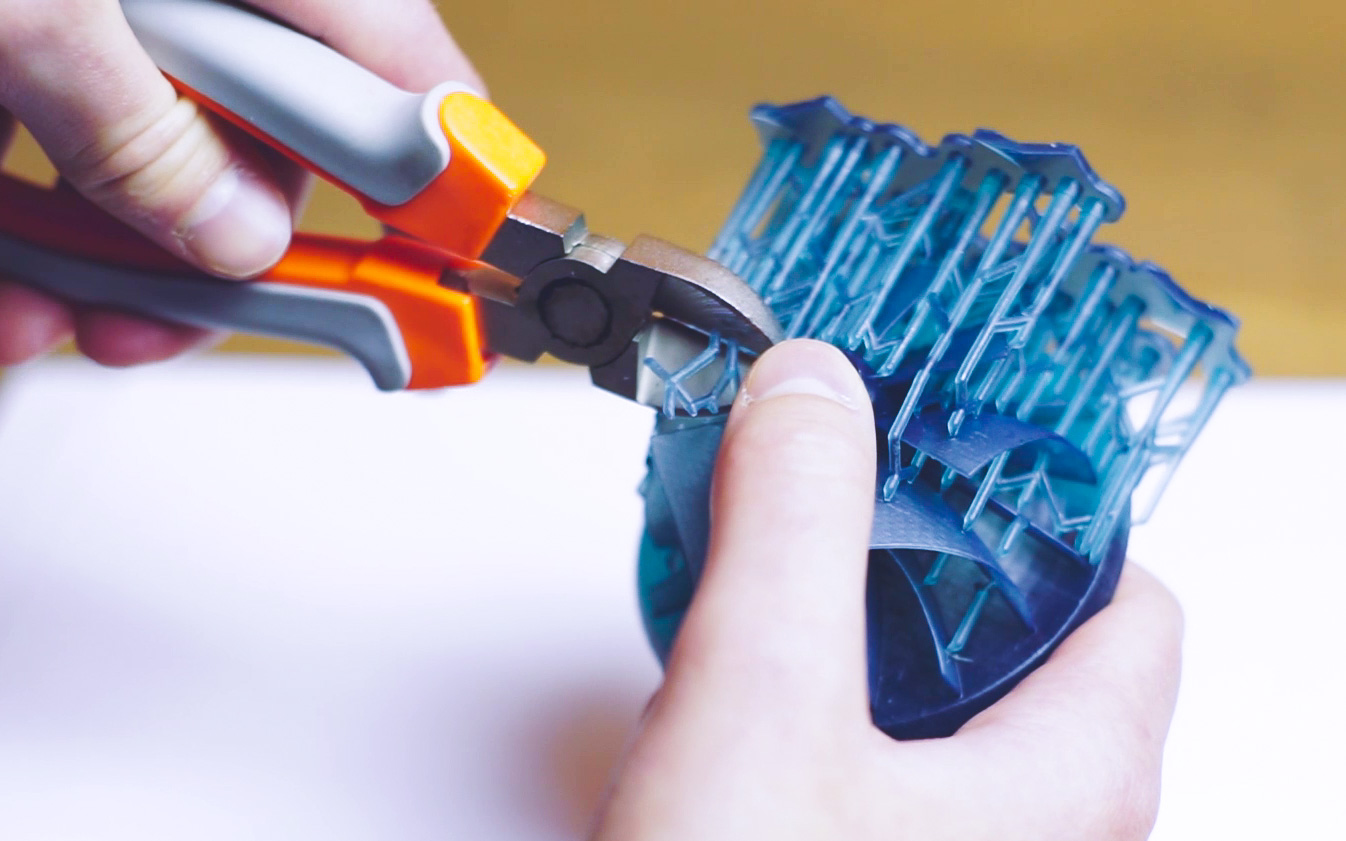
\includegraphics[height=5cm]{illustration-supports}
\caption{Illustration des supports d'impression 3D}
\end{figure}

L'avantage d'avoir des supports interne est avant tout que ceux-ci peuvent accroître la solidité du modèle, et également que ceux-ci ne sont pas obligatoirement à retirer. L'algorithme de grassfire transform permet la création de support interne nécessitant très peu de matière. Cet algorithme est actuellement implémenté dans IceSL. Il nécessite au préalable l'extraction de l'axe médian pour chacune des slice de chaque modèle soumis à l'impression, ce qui est la majeure partie du coup de l'algorithme. Le nombre de slice croissant rapidement avec la taille de l'objet et avec le détail désiré, il devenait nécessaire de posséder un algorithme de calcul d'axe médian rapide et efficace.Il s'agit ici du cadre de ce projet.


\section{Algorithme de support interne, intérêt du projet}

\subsection{L'axe Median}

Une notion centrale dans ce document est l'axe médian d'une forme geométrique\footnote{Forme en 2D uniquement dans le cadre de ce projet, hypothèse non limitante}. Instinctivement, l'axe médian est le squelette d'une forme connexe, au sens où on l'entend, la forme connexe étudiée étant une peau et l'intérieur le squelette de la forme.

\begin{figure}[h]
\centering
\includegraphics[ trim = {0 0 0 9cm}, clip, height=3cm]{medial-axis}
\caption{Examples instinctif de contours et de leur axe médian}
\end{figure}

Mathématiquement, l'axe médian se définit de la manière suivante :
\vspace{5mm}
\begin{changemargin}{2cm}{2cm}
\it Soit $C$ un ensemble de points formant un contour, alors l'axe médian est l'ensemble des centre dec boules contenues dans C tangeantes à C en au moins 2 points.

\end{changemargin} 

\subsection{Algorithme de Grassfire transform}

Pour chacune des slices effectuées pour l'impression 3D, on extrait leur axe médian respectif, indépendamment les unes des autres.
\paragraph*{}
L'algorithme de grassfire transform est un algorithme à effectuer avant l'impression, afin de calculer les supports à imprimer. L'algorithme se fait slice par slice, indépendamment les unes des autres, en partant de la slice la plpus haute. On itère sur ce qu'on imprime en creusant afin d'imprimer le moins de matière possible.

À l'itération zéro, on imprime tout le modèle en bloc. Chaque itération se fait sur la totalité du modèle. 

\paragraph*{} Pour une slice $n$ donnée :
\begin{itemize}
\item On extrait l'axe médian.
\item On \textit{creuse} dans le modèle (c'est à dire on dilate la cavité non imprimée) à partir de la cavité précédente et de la portion d'axe médian à la slice $n-1$. comme montré dans l'exemple suivant.
\end{itemize}

\section{L'extraction de l'axe médian : coeur du projet}

\subsection{Modélisation du contour}

Le contour dont nous souhaitons extraire l'axe médian est assimilé à un nuage de point, discrétisé. Il sera représenté par un membre de la classe <Graph>. La classe dispose d'une fonction premettant d'augmenter la densité de point du graphe, qui sera utile pour la suite.

La classe graphe possède différents attributs \begin{itemize}
\item le vector contenant les coordonnées de chaque point, où l'index de chaque point est son emplacement dans le vecteur de coordonnées

\item Une liste d'adjacence contenant pour chaque point, la liste des indices des points qui lui sont relié par une arête.
\end{itemize}

\vspace{8mm}

Pour le graphe représentant le diagramme de voronoi (aussi représenté utilisant la classe Graph), nous avons besoin de plus d'information afin d'effectuer les étapes de filtrage nécessaire : 
\begin{itemize}
\item Un vecteur \texttt{pointTreatment} donnant le traitement de chaque point, représenté par un enum : \texttt{outside, inside} ou \texttt{unknown}.
\item Les arêtes ne sont pas stockées de la même manière, car il est important dans le cadre du grassfire transform de conserver la point du contour le plus proche de la portion d'axe médian. Pour cela, la liste d'adjacente est une liste de \texttt{struct Neighbor} contenant l'indice du point de destination de l'arête, ainsi que les coordonnées du point du contour le plus proche de l'arête considérée.
\end{itemize}

\begin{figure}
\centering
\includegraphics[width = 15cm]{classe-graph}
\caption{Structure de la classe graph}
\end{figure}


\subsection{La triangulation de delaunay}

\subsubsection{Définition et example}

La triangulation de delaunay forme des triangles avec le nuage de points tel que tous les cercles circonscrits des triangles ne contiennent aucun point du nuage.

\begin{figure}[h]
\centering
\includegraphics[height=6cm]{delaunay-ex}
\caption{Un exemple de triangulation de delaunay}
\end{figure}

La triangulation de delaunay est donc un calcul sur un nuage de point et non sur un contour, comme il est l'étape une de notre algorithme, il est nécessaire que les nuage de points embrassent au plus proche possible la structure de contour, et c'est dans ce cadre que la fonction d'augmentation de densité sera primordiale.


\subsubsection{Une première étape du projet}
La triangulation de delaunay est la première étape du programme, de laquelle nous partons. Nous utilisons la librairie GEOGRAM développée par Bruno Levy, dans laquelle il suffit de donner en entrée un ensemble de points, et la triangulation de delaunay est alors calculée. 

\paragraph*{}
Il y a plusieurs raisons pour lesquelles ce calcul est effectuée par une librairie tierce :
\begin{itemize}
\item Les calculs sur les flottants peuvent s'avérer très complexe, et un algorithme calculant effectivement la triangulation de delaunay est extrêmement difficile à faire
\item Le cadre du projet nécessite la triangulation de delaunay, qui est ici obtenue de manière optimale, aucune raison de réinventer la roue.
\end{itemize}



\subsection{Le dual de la triangulation de delaunay : le diagramme de voronoi}

Afin d'obtenir le diagramme de voronoi du contour, dont l'axe médian sera un sous ensemble, il faut prendre tous les centre des cercles circonscrit aux triangles de delaunay, et les relier en traçant les perpendiculaires aux côtés des triangles, on obtient alors le graphe dual, c'est à dire le diagramme de voronoi. On voit la triangulation en noir, et son dual en rouge, sur la figure 5.

 \begin{figure}[h]
\centering
\includegraphics[height=6cm]{voronoi-del}
\caption{Un exemple de diagramme de voronoi obtenu à partir de la triangulation de delaunay}
\end{figure}

Pendant le calcul du diagramme de voronoi, il est important de noter si un edge traverse la surface que nous souhaitons imprimer, car c'est le seul endroit où cette information sera accessible de manière simple. Pour ce test, il suffit de regarder si l'arête du diagramme de delaunay que nous regardons est également une arête du contour à imprimer, comme l'arête de voronoi correspondante la traversera nécessairement et uniquement, on saura si l'arête de voronoi traverse la surface. 

\paragraph*{}
L'extraction de la triangulation de delaunay étant effectuée par GEOGRAM, l'extraction de voronoi est faite directement, en une seule fonction.




\subsection{Passage du diagramme de voronoi à l'axe médian}

L'axe médian correspond au diagramme de voronoi auquel on a supprimé tous les points extérieur au contour à imprimer. Il y a donc deux étapes à effectuer afin de supprimer ces points sans effectuer trop de calculs : 
\begin{itemize}
\item Déterminer certain points dont la position est connue.
\item Parcourir le graphe avec sachant pour chaque arête si elle coupe le contour, afin de propager l'information inside/outside
\end{itemize}


\subsubsection{Déterminer les points dont la position relative au contour est connue}
Pour plus de clarté, dans la suite, nous noterons \emph{traitement} pour décrire le status inside/outside d'un point du diagramme de voronoi. Certains points du diagramme de voronoi se retrouvent à l'infini, par construction. En regardant l'arête qui relie le point à l'infini avec le point de coordonnées bornées, avec l'information des arêtes traversant la surface, il est possible de déterminer le traitement du point considéré. Le point à linfini étant nécessairement dehors, le point considéré et inside si l'edge croise la surface et outside sinon.

\subsubsection{Propagation de l'information et supression}

L'information se propage alors via un parcours en profondeur, en veillant bien à ne parcourir une seule fois chaque vertex du diagramme de voronoi. Une fois l'information propagé sur chaque point du graphe, il faut alors supprimer les points étant hors du contour. 

\paragraph*{}
L'un des aspect les plus important est de garder le moins d'opération possible, la suppression est alors effectuée en échangeant les index à garder et les index à supprimer dans les liste d'ajacence et dans le vecteur de coordonnées.

\section*{Conclusion}

Ce projet nous a appris une certaine critique sur l'aspect mathématique des données de par sa liberté dans leur modélisation. Il nous a également appris à nous questionner sur la robustesse de l'algorithme dans de nombreuses fonctions, notamment sur certains cas à problème qui doivent fonctionner correctement, car nous ne serons pas là pour faire de la maintenance. Enfin ce projet nous a appris le C++, langage que nous ne maîtrisions pas.

\paragraph*{}
Le code produit sera implémenté dans la dernière version d'IceSL prochainement et il s'agit d'un grand accomplissement d'être cité dans un tel projet pour deux élèves d'école d'ingénieur.

\end{document}
\grid